\section{Установления взаимосвязей между новостями и твитами}
    Задача автоматического установления связей между твитами и новостями решена посредством написания программного комплекса,
    который обладает следующими возможностями:
    \begin{enumerate}
        \item сбор необходимой для решения задачи информации;
        \item получение рекомендаций новостей для произвольных твитов;
        \item вариативность в выборе метода для построения рекомендаций;
        \item возможность получить информацию о качестве используемого метода.
    \end{enumerate}
    Поставленная задача достигается за счёт реализации отдельных преобразований над данными в рамках написанного программного комлекса
    с использованием языка программирования Python версии 2.7.
    Далее приводится описание реализованных преобразований и подробный разбор отдельных моментов.


    \subsection{Архитектура}
    Программный комплекс позволяет производить все требуемые для решения задачи преобразования над данными, а именно:
    \begin{enumerate}
        \item получение данных из твиттера;
        \item получение данных из новостной rss-ленты;
        \item расшифровка сокращённых URL;
        \item автоматическое построение набора данных;
        \item построение моделей для методов WTMF и WTMF-G;
        \item построение рекомендаций на основе методов WTMF, WTMF-G и TF-IDF;
        \item оценка качества рекомендаций;
        \item получение результатов рекомендаций в пригодном для чтения формате;
    \end{enumerate}
%    Результаты всех преобразований, за исключением оценки качества и получения рекомендаций, хранятся в специальном промежуточном
%    хранилище~(побробное описания хранилища производится в разделе~\ref{sec:documentation}).

    Каждое преобразование, в общем случае, независимо от других.
    Для построения рекомендаций, необходимо выполнить цепочку преобразований.
    Примеры цепочек преобразований для получения данных, построения рекомендаций и оценки их качества приводятся ниже.
    
    Визуализация цепочек преобразований производится при помощи рисунков, использующих элементы блок-схем~\cite{flowchart_gost}.
    Для удобства восприятия блоки действия~(изображаются прямоугольником) выделяются зелёным цветом, 
    а прочие используемые блоки, такие как ввод-вывод данных~(изображаются параллелограммом) и хранимые 
    данные~(изображаются фигурой, представляющей собой прямоугольник, в котором две противолежащие стороны 
    заменены на две одинаковые и параллельные кривые, совпадающие с секцией окружности), выделяются синим цветом.
    
    Получение данных заключается в скачивании новостей из RSS потоков и твитов, с использованием Twitter Streaming API, в течение длительного промежутка времени, с последующим помещением всех данных в промежуточное хранилище. В работе в качестве хранилища выступает python shelve.
    Получение данных в виде блок-схемы изображен на рисунке~\ref{pic:consumer_flowchart}.
    \begin{figure}[h!]
            \center
            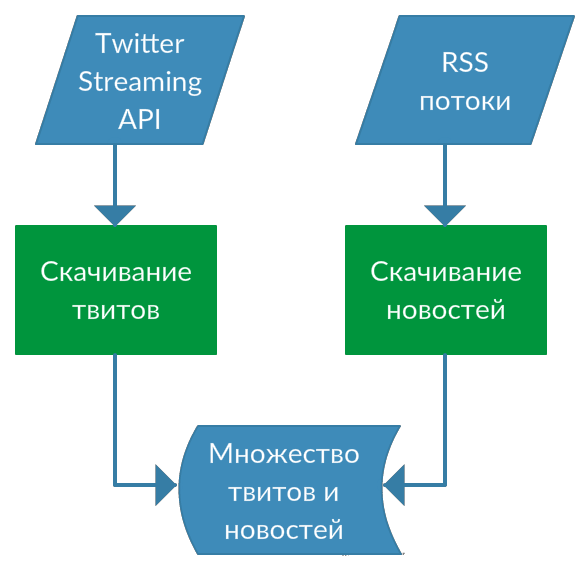
\includegraphics[scale=0.4]{twnews_consumer_flowchart.png}
            \caption{Блок-схема получения данных}
            \label{pic:consumer_flowchart}
    \end{figure}

    На основе полученного множества новостей и твитов происходит автоматическое построение набора данных. В рамках автоматического построения набора данных происходит расшифрка сокращённых URL.
    Набор данных эта структура состоящая из списка новостей и списка твитов, где для каждого твита указана ссылка на единственную новость.

    Результатом работы всех реализованных методов является сопоставление численных векторов~(векторов для сравнения) каждому обрабатываемому тексту, с помощью которых можно оценить насколько похожи любые два текста. 

    Метод TF-IDF не имеет стадии обучения модели, поэтому применяется непосредственно к набору данных и получает вектора для сравнения, для всех текстов, которые были переданы ему на вход.
    Получаемые векторы обладают размерностью совпадающей с размером корпуса.

    В отличие от метода TF-IDF методы WTMF и WTMF-G состоят из двух стадий: обучения и применения модели. На стадии обучения методы строят модель~(в сериализованной модели помимо самой модели содержится набор данных, на основе которого была построена модель) и получают вектора для сравнения для всех элементов набора данных. На стадии применения методы WTMF и WTMF-G на основе ранее построенной модели для произвольного множества твитов строят векторы для сравнения полученных на вход твитов и новостей из набора данных.

    На основе множества, состоящего из твитов и новостей, для каждого элемента в котором существует вектор для сравнения, строятся рекомендации.
    Рекомендации представляют собой множество твитов, к каждому из которых сопоставлен ранжированный по мере убывания схожести список новостей.

    \begin{figure}[h!]
            \center
            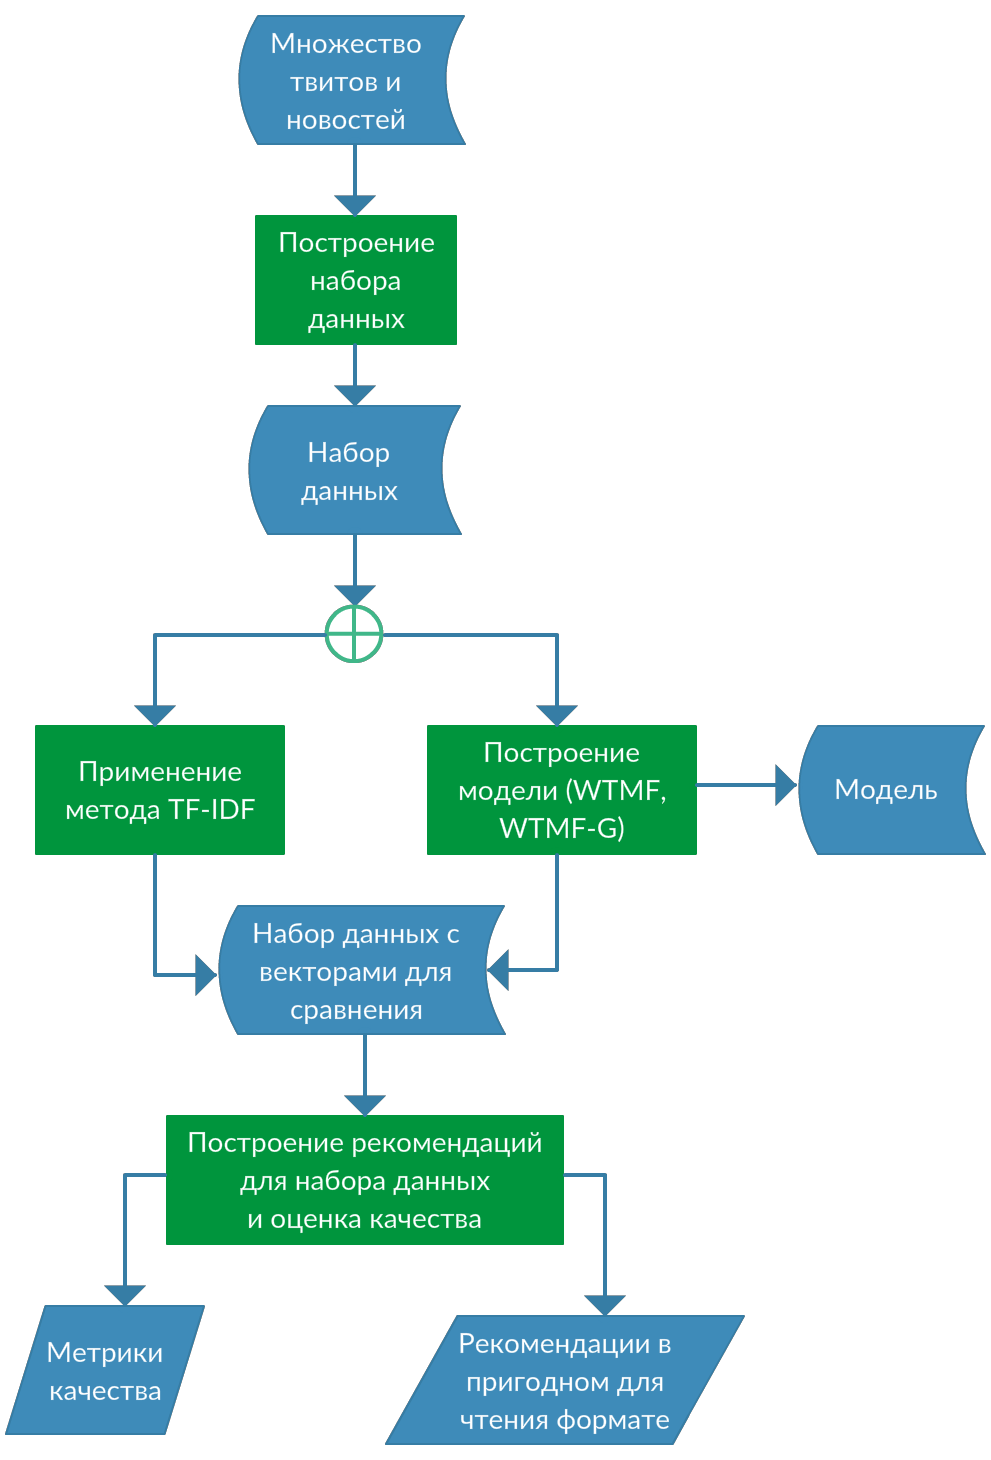
\includegraphics[scale=0.32]{twnews_flowchart_1.png}
            \caption{Блок-схема процесса оценки качества используемых методов}
            \label{pic:twnews_flowchart_1}
    \end{figure}

    На основе построенных рекомендаций можно как произвести оценку качества ранее использованного метода, так и получить их в виде текстового файла,
    который содержит информацию в пригодном для чтения формате.
    Оценка качества использованного метода производится при условии построения рекомендаций для набора данных.
    Процесс оценки качества различных методов рекомендаций, а также получение рекомендаций для твитов из набора данных изображён на рисунке~\ref{pic:twnews_flowchart_1}.

    Дополнительным результатом изображённого на рисунке~\ref{pic:twnews_flowchart_1} процесса является построенная модель (для методов WTMF и WTMF-G), которую можно применить на произвольное множество твитов. Процесс получения рекомендаций для произвольных твитов изображён на рисунке~~\ref{pic:twnews_flowchart_2}.
    
    \begin{figure}[h!]
            \center
            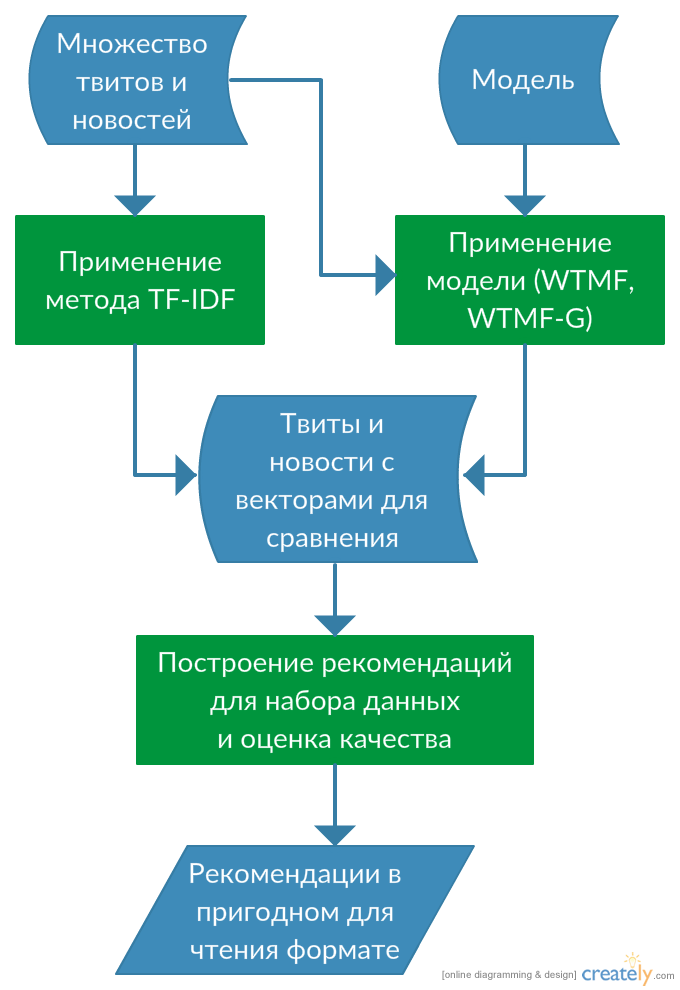
\includegraphics[scale=0.32]{twnews_flowchart_2.png}
            \caption{Блок-схема процесса получения рекомендаций для различных методов}
            \label{pic:twnews_flowchart_2}
    \end{figure}

    %\textcolor{red}{заключительный абзац}

    




    \subsection{Nature Language Processing}
    Всё что связано с обработкой текста

    \subsubsection{Лемматизация}
    \label{subsubsec:lemma}
        что это

        как используется

        https://pythonprogramming.net/stop-words-nltk-tutorial/?completed=/tokenizing-words-sentences-nltk-tutorial/
    \subsubsection{Извлечение имён собственных}
        что это

        Обзор подходов

        объяснение используемого

    \subsection{Метод WTMF}
    Модель для метода WTMF построена на основе мнзаранее подготовленного набора данных.
    В контексте работы набор данных состоит из множества новостей и твитов, из которых в процессе работы извлекается набор текстов
    ~(для твита~---~текст твита, для новости~---~конкатенация заголовка и краткого изложения статьи).

    По множеству текстов, которые получены из набора данных, построена модель, пригодная для сериализации, состоящая из матрицы $P$
    ~(здесь и далее используются обозначения введённые в главе \ref{subsubsec:wtmf}).
    Построение модели зависит от четырёх констант:
    \begin{enumerate}
        \item $K$~---~размерность вектора, по которому производится сравнение~
        (если TF-IDF матрица $X$ была размера $M \times N$, то по завершении работы алгоритма будут получены две матрицы $P$ размера $K \times M$ и $Q$ размера $K \times N$);
        \item $I$~---~число итераций алгоритма построения модели;
        \item $w_M$~---~коэффициент, задающий вес негативного сигнала при построении матрицы весов $W$;
        \item $\lambda$~---~регуляризирующий член.
    \end{enumerate}

    Применение полученной модели на множество твитов представляет собой следующий процесс:
    сначала строится TF-IDF матрица $X$ для новостей из набора данных и множества твитов, затем на основе новой матрицы $X$ строится весовая матрица $W$,
    и наконец на основе построенных матриц $X$ и $W$ и посчитанной на этапе обучения матрицы $P$ выполняется половина итерации алгоритма обучения,
    а именно получение матрицы $Q$ по матрице $P$:
    $$Q_{\cdot, j} = (P W'_j P^T + \lambda I)^{-1} P W'_j X_{j,\cdot}.$$
    В результате получаем вектора для сравнения твитов из заданного множества.
    \subsection{Метод WTMF-G}
    Построение модели для метода WTMF-G основывается на построение модели метода WTMF.
    Набор данных состоит из множества новостей и твитов и связей вида текст-текст, из которых, в процессе работы извлекается набор текстов.
    ~(для твита~---~текст твита, для новости~---~конкатенация заголовка и краткого изложения статьи).

    По множеству текстов, которые получены из набора данных, построена пригодная для сериализации модель, представляющая собой матрицу $P$.
    Построение модели зависит от четырёх констант:
    \begin{enumerate}
        \item $K$~---~размерность вектора, по которому производится сравнение~
        (если TF-IDF матрица $X$ была размера $M \times N$, то по завершении работы алгоритма будут получены две матрицы $P$ размера $K \times M$ и $Q$ размера $K \times N$);
        \item $I$~---~число итераций алгоритма построения модели;
        \item $w_M$~---~коэффициент, задающий вес негативного сигнала при построении матрицы весов $W$;
        \item $\delta$~---~коэффициент, задающий степень влияния связей вида текст-текст.
    \end{enumerate}

    Применение полученной модели на множество твитов производится аналогично применению модели для метода WTMF за исключением двух моментов:
    во-первых, необходимо на основе новостей из набора данных и множества твитов перестроить связи текст-текст, во-вторых получение матрицы $Q$ происходит по следующей формуле:
    $$Q_{\cdot, j} = (P W'_j P^T + \lambda I + \delta  L_j^2 Q_{\cdot,n(j)} diag(L^2_{n(j)})Q_{\cdot,n(j)}^T)^{-1}   (P W'_j X_{j,\cdot} + \delta  L_j Q_{\cdot,n(j)} L_{n(j)}).$$
    В результате получаем вектора для сравнения твитов из заданного множества.
    
\subsection{Эффективная работа с матрицами}
    Построение и применение моделей WTMF и WTMF-G требует большого количества операций над матрицами, что на практике занимает продолжительное время.
    Поэтому задача по повышению эффективности работы с матрицами актуальна.

    Для эффективной работы с матрицами используются программные библиотеки для языка Python numpy и
    scipy~(базируется на библиотеке numpy и расширяет её функционал).

    Оптимизируется формула получения строк матрицы $P$, используемая при построении моделей WTMF и WTMF-G.
    На каждой итерации построения модели происходит многократное выполнение формулы (количество выполнений порядка $10^4$, зависит от размера корпуса):
    $$P_{i, \cdot} = (Q W'_i Q^T + \lambda I)^{-1} Q W'_i X_{i,\cdot}^T.$$

    В начале была написана наивная реализация алгоритма, которая показала производительность, не приемлемую в рамках решения задачи.
    Затем наивная реализация оптимизировалась следующим образом:
    \begin{enumerate}
        \item переход к перемножению матриц с использованием высокопроизводительной библиотеки для языка С OpenBlass~(в библиотеке numpy существует возможность перейти к использованию для работы с матрицами некоторых библиотек, написанных на языке С~\cite{blas_installation});
        \item сохранение в отдельной переменной переиспользуемых результатов вычислений над матрицами;
        \item переписывание кода для работы с разреженными матрицами;
        \item удаление лишних приведений матриц к формату python list и обратно.
    \end{enumerate}
    Результаты оптимизации приведены в таблице~\ref{tabular:matrix_optimization}.

    \begin{table}[ht!]
        %\small
        \caption{Оптимизация работы с матрицами\bigskip}
        \centering

        \label{tabular:matrix_optimization}
        \begin{tabular}{|p{5cm}|c|c|}
            \hline
            \bf{\specialcell{Добавленная \\ оптимизация}} &
            \bf{\specialcell{Время за \\ 100 итераций~(c)}} &
            \bf{\specialcell{Прирост \\ производительности \\ (раз) }} \\ \hline

            Наивная реализация & 205 & 1 \\ \hline
            Перемножение с помощью OpenBlass & 55 & 3.73 \\ \hline
            Переиспользование результатов & 15.15 & 3.63 \\ \hline
            Работа с разреженными матрицами & 0.75 & 20.2 \\ \hline
            Сокращение количества приведений типов & 0.63 & 1.21 \\ \hline
        \end{tabular}
    \end{table}
    Получили, что оптимизированное решение работает в 325 раз быстрее наивной реализации.
    Дальнейшая оптимизация не производилась, так как получено решение работающее за приемлемое время.
%    Дополнительную оптимизацию можно произвести с помощью использования библиотек для работы с матрицами, использующих видеокарт
%
%
%
%    идеи по дальнейшей оптимизации: CUDA

